\chapter{ثبات الجينوم: أذية DNA وإصلاحه وإعادة التركيب}\label{ch:b3:dna-repair}

تضع ظهيرة على شاطئ نحو مئة ألف آفة كيميائية في DNA كل خلية جلدية
معرَّضة للشمس: ثيمينان متجاوران يُلحمان ثنائيًا بالأشعة فوق البنفسجية،
وقواعد تتأكسد، وطاقات تُثلم. ومن غير شمس البتة، يخلع ماء الخلية
الدافئ نحو عشرة آلاف بورين عن سكرياتها كل يوم ويحوّل مئات
السيتوزينات إلى يوراسيل. ومع ذلك فمعدل الطفرة في الخلية البشرية نحو
تغير واحد في كل عشرة مليارات زوج قواعد لكل انقسام --- أي في جينوم
من ستة مليارات، أقل من طفرة جديدة واحدة في الانقسام. والفجوة بين ما
يصيب الجينوم من أذًى وما يبقى فيه منه يسدها الإصلاح: عشرات من منظومات
الإنزيمات تجوس اللولب المزدوج، وتتعرف ما لا ينبغي أن يكون فيه،
فتستأصله وتعيد البناء عن الطاق السليم، وإذا انكسر الطاقان معًا
وصلتهما أو نسخت القطعة الناقصة عن شقيقة. والأطفال الذين تنقصهم إحدى
هذه المنظومات --- يحترقون عند أول مسّ من ضوء الشمس، أو يصابون بسرطان
القولون في ثلاثينياتهم --- يبينون ما تساويه هذه المنظومات. وهذا الفصل
عن الأذية، ومسالك الإصلاح، وآلة إعادة التركيب التي تصلح أسوأ الكسور
والتي يستعيرها الانقسام المنصّف، وقرار الخلية حين يخفق الإصلاح: أن
تكفّ عن الانقسام أو أن تموت.

\section{ما الذي يصيب DNA}

\begin{definition}[آفات DNA]\label{def:b3:dna-repair:lesions}
\index{آفة DNA}\index{نزع البورين}\index{نزع الأمين}\index{ثنائي البيريميدين}\index{كسر مزدوج الطاق}\index{8-أوكسوغوانين}
\emph{الآفة} أي تبدل كيميائي في DNA يبعده عن القواعد الأربع السوية
مزدوجةً ازدواجًا صحيحًا على هيكل سليم. وتنشأ الآفات العفوية من كيمياء
الماء والأكسجين: \emph{نزع البورين}، وهو حلمهة الرابطة بين البورين
وسكره فيبقى موضع بلا قاعدة (نحو $10^{4}$ في الخلية كل يوم)؛ و\emph{نزع
الأمين}، الذي يحوّل السيتوزين إلى يوراسيل، و5-ميثيل سيتوزين إلى
ثيمين، والأدنين إلى هيبوكسانثين (بضع مئات في اليوم)؛ و\emph{الأكسدة}
بأنواع الأكسجين الفعالة، وأشهر نواتجها \emph{8-أوكسوغوانين}، الذي
يزدوج مع الأدنين بسهولة ازدواجه مع السيتوزين؛ و\emph{أخطاء
التضاعف}، من قاعدة أُدخلت خطأً أو انزلقت. أما الآفات البيئية فمنها
\emph{ثنائي البيريميدين الحلقي البوتاني} والناتج الضوئي 6-4 اللذان
يصنعهما الضوء فوق البنفسجي بين بيريميدينين متجاورين؛ والقواعد
المؤلكلة من العوامل المؤلكلة (فالغوانين O$^{6}$-الميثيل
يزدوج مع الثيمين)؛ والملحقات الضخمة من الهدروكربونات العطرية
والأفلاتوكسين؛ والتشابكات بين الطاقين من السيسبلاتين وخردل
النتروجين؛ والكسور مفردة الطاق و\emph{مزدوجة الطاق}
التي يصنعها الإشعاع المؤيّن، نحو \num{1000} كسر مفرد و
\numrange{30}{40} كسر مزدوج في الخلية لكل غراي.
\end{definition}

\begin{proposition}[سلّم الأمانة]\label{prop:b3:dna-repair:fidelity}
\index{أمانة}\index{تدقيق}\index{إصلاح عدم التوافق}
يبلغ التضاعف معدل خطئه البالغ نحو $10^{-10}$ لكل زوج قواعد في ثلاث
خطوات متضاعِفة. فانتقاء القاعدة بالبوليميراز، اعتمادًا على الهندسة
والروابط الهدروجينية، يخطئ نحو مرة في $10^{5}$؛ و\emph{التدقيق}
بالنوكلياز الخارجي 3$'\to$5$'$ في البوليميراز، الذي يستأصل قاعدة
طرفية غير مزدوجة قبل الاستطالة، يزيل \qty{99}{\%} منها؛ و\emph{\omterm{prop:b3:dna-repair:fidelity}{إصلاح
عدم التوافق}}، العامل خلف الشوكة على الطاق المصنوع حديثًا، يزيل
\qty{99.9}{\%} مما بقي. والجداء
$10^{-5}\times 10^{-2}\times 10^{-3} = 10^{-10}$ هو المعدل المرصود،
وأي خلل في إحدى خطوتي التصحيح يرفعه مئة ضعف أو ألف ضعف: وتسمى تلك
الخلايا \emph{مطفِّرات}.
\end{proposition}

\begin{example}[الآفات في مقابل الطفرات]\label{ex:b3:dna-repair:numbers}
الخلية البشرية ذات $6.4\times 10^{9}$ زوج قواعد المنقسمة مرة في اليوم
تتراكم فيها آفات في حدود $10^{4}$--$10^{5}$ في اليوم و
نحو $6.4\times 10^{9}\times 10^{-10} \approx 0.6$ طفرة جديدة في
الانقسام: فلا تنجو آفة واحدة من كل عشرة آلاف لتصير تغيرًا دائمًا.
أما الباقي فيُصلَح قبل أن يقرأه التضاعف، ومعدل النجاة إلى طفرة ---
لا معدل الأذية --- هو ما صغّره الانتقاء. والحساب نفسه يبين لماذا يَعُدّ
عددُ الطفرات في ورم أو في نطاف أب متقدم في السن الانقساماتِ: فطفرات
الخلية هي، بالتقريب الأول، عدد انقساماتها مضروبًا في الخطأ في الانقسام.
\end{example}

\section{إصلاح طاق واحد متأذٍّ}

\begin{definition}[إصلاح الاستئصال]\label{def:b3:dna-repair:excision}
\index{إصلاح استئصال القاعدة}\index{إصلاح استئصال النوكليوتيد}\index{غليكوزيلاز}\index{جفاف الجلد المصطبغ}
تصيب معظم الآفات طاقًا واحدًا، وتُصلَح بقطع الجزء المتأذي ونسخ الطاق
الآخر. و\emph{إصلاح استئصال القاعدة}
(BER) يعالج الآفات الصغيرة غير المشوِّهة: إذ يقلب \emph{غليكوزيلاز DNA}
خاص بنوع واحد من القواعد الخاطئة (غليكوزيلاز اليوراسيل، وغليكوزيلاز
\omterm{def:b3:dna-repair:lesions}{8-أوكسوغوانين}، وغيرهما) القاعدةَ خارج اللولب ويقصّها عن سكرها؛
وينثلم نوكلياز داخلي AP الهيكلَ عند الموضع بلا قاعدة؛ ويزيل
بوليميراز (Pol~$\beta$) السكر ويدخل نوكليوتيدًا واحدًا؛ ويختم ليغاز.
و\emph{إصلاح استئصال النوكليوتيد}
(NER) يعالج الآفات الضخمة المشوِّهة للولب --- ثنائيات البيريميدين
والملحقات الكيميائية --- من دون أن يتعرف كيمياء \omterm{def:b3:dna-repair:lesions}{الآفة}
نفسها: إذ يُكشف التشويه (ببروتين XPC الماسح للجينوم، أو ببوليميراز
RNA متوقف في الفرع المقترن بالاستنساخ)، ويُفتح
اللولب بوحدات الهليكاز في TFIIH، ويُتحقق من الأذية (XPA)،
ويقطع نوكليازان داخليان (XPF وXPG) الطاق المتأذي
على بعد \numrange{24}{32} نوكليوتيدًا، ويُطلق قليل النوكليوتيد،
ويملأ البوليميراز والليغاز الفجوة. وفقدُ أي من بروتينات
XP السبعة يسبب \emph{جفاف الجلد المصطبغ}: حساسية مفرطة لضوء
الشمس، ونمش، ومعدلُ سرطان جلد أعلى بألف ضعف.
\end{definition}

\begin{proof}[شواهد]
زرع كليفر (1968) خلايا جلدية ليفية من مرضى \omterm{def:b3:dna-repair:excision}{جفاف الجلد المصطبغ}،
وشعّعها بالضوء فوق البنفسجي وأعطاها ثيميدينًا مشعًا خارج الطور S.
فأدخلت الخلايا السوية الواسمَ في مواضع صغيرة كثيرة --- وهو ``تركيب
DNA غير المجدول'' في رقع الإصلاح --- بينما لم تُدخل خلايا المرضى شيئًا
يُذكر، وماتت عند جرعات نجت منها الخلايا السوية: فالمرض إخفاق في
استئصال الثنائيات. وكان دمج خلايا من مريضين يعيد الإصلاح في الهجين
غالبًا، إذ يمدّ كل منهما الآخر بما ينقصه؛ وبهذا المحك فُرز المرضى إلى
زمر تتام من A إلى G، زمرة لكل مورّثة من مورّثات المسلك، قبل استنساخ
المورّثات بسنين.
\end{proof}

\begin{omfigure}
\begin{tikzpicture}[every node/.style={font=\scriptsize}, >=stealth]
  % BER column
  \node[font=\small\bfseries] at (2.0,3.2) {إصلاح استئصال القاعدة};
  \foreach \y/\txt in {2.6/{قاعدة متأذية (U، 8-أوكسوغوانين)}, 1.5/{الغليكوزيلاز يزيل القاعدة}, 0.4/{نوكلياز AP الداخلي يثلم}, -0.7/{Pol $\beta$ يملأ نوكليوتيدًا واحدًا، والليغاز يختم}} {
    \draw[very thick, omDef] (0.2,\y) -- (3.8,\y); \draw[very thick, omDef] (0.2,\y-0.25) -- (3.8,\y-0.25);
    \node[right, align=left] at (0.2,\y-0.6) {\txt};
  }
  \fill[omThm] (2.0,2.6) circle (0.1);
  \draw[omThm, thick] (1.9,1.5) -- (2.1,1.5);
  \draw[white, very thick] (1.9,0.4) -- (2.1,0.4);
  \fill[omMeth!80!black] (2.0,-0.7) circle (0.1);
  % NER column
  \node[font=\small\bfseries] at (8.0,3.2) {إصلاح استئصال النوكليوتيد};
  \foreach \y/\txt in {2.6/{آفة ضخمة تشوّه اللولب؛ XPC يرتبط}, 1.5/{TFIIH يفتح اللولب، وXPA يتحقق}, 0.4/{XPF وXPG يقطعان على بعد 24--32 نوكليوتيدًا}, -0.7/{البوليميراز يملأ الفجوة، والليغاز يختم}} {
    \draw[very thick, omDef] (6.2,\y) -- (9.8,\y); \draw[very thick, omDef] (6.2,\y-0.25) -- (9.8,\y-0.25);
    \node[right, align=left] at (6.2,\y-0.6) {\txt};
  }
  \draw[omThm, very thick] (7.8,2.6) -- (8.2,2.6) -- (8.2,2.75) -- (7.8,2.75) -- cycle;
  \draw[omDef, very thick] (7.2,1.5) .. controls (7.6,1.85) and (8.4,1.85) .. (8.8,1.5); \draw[omThm, very thick] (7.85,1.72) -- (8.15,1.72);
  \draw[very thick, white] (7.0,0.4) -- (9.0,0.4); \draw[omThm, thick, ->] (7.0,0.7) -- (7.0,0.48); \draw[omThm, thick, ->] (9.0,0.7) -- (9.0,0.48);
  \draw[very thick, omMeth!80!black] (7.0,-0.7) -- (9.0,-0.7);
\end{tikzpicture}

{\small مسلكا استئصال. يتعرف استئصال القاعدة (يسارًا) قاعدةً خاطئة
بعينها \omterm{def:b3:dna-repair:excision}{بغليكوزيلاز} مخصص ويستبدل نوكليوتيدًا واحدًا. ويتعرف استئصال
النوكليوتيد (يمينًا) التشويهَ الذي تحدثه أي آفة ضخمة، فيقطع الطاق من
جانبيه ويستبدل رقعة من نحو ثلاثين نوكليوتيدًا (بالأخضر).}
\end{omfigure}

\begin{definition}[إصلاح عدم التوافق]\label{def:b3:dna-repair:mmr}
\index{إصلاح عدم التوافق!تمييز الطاق}\index{متلازمة لينش}\index{عدم استقرار السواتل المكروية}
\emph{\omterm{prop:b3:dna-repair:fidelity}{إصلاح عدم التوافق}} (MMR) يصحح الأزواج الخاطئة وعرى الإقحام
والحذف الصغيرة التي تفلت من التدقيق. فبروتين MutS
(MSH2--MSH6 في البشر) يتعرف تشويه عدم التوافق، ويرخّص مع
MutL (MLH1--PMS2) لنوكلياز خارجي أن يحلل الطاق المصنوع
حديثًا من ثلمة قريبة رجوعًا إلى ما بعد موضع عدم التوافق؛ ثم يملأ
البوليميراز الفجوة. والصعوبة هي \emph{تمييز الطاق}: فلعدم التوافق
قاعدتان وواحدة منهما فقط هي الخاطئة. وفي
\emph{Escherichia coli} يُعرف الطاق الجديد لأنه لم
يُمثيل بعدُ عند مواقع GATC التي تعلّمها ميثيلاز Dam بعد التركيب ببضع
دقائق؛ فينثلم MutH الطاقَ غير الممثيل. وفي
حقيقيات النوى يُعرف الطاق الجديد بالثلمات بين قطع أوكازاكي
وبالنهاية 3$'$ الحرة في الطاق القائد. وفقد MMR
يرفع معدل الطفرة مئة إلى ألف ضعف، وأظهر ما يكون ذلك
عند \emph{السواتل المكروية} --- وهي أشواط من تكرار قصير ينزلق فيها
البوليميراز --- إذ تتغير أطوالها من خلية إلى خلية: وهو
\emph{عدم استقرار السواتل المكروية}. وفقدُ أليل واحد من MMR وراثةً هو
\emph{متلازمة لينش}، مع سرطان قولون ومستقيم في نحو \qty{70}{\%} من
الحاملين، وقبل الخمسين غالبًا.
\end{definition}

\begin{omfigure}
\begin{tikzpicture}[every node/.style={font=\scriptsize}, >=stealth]
  \draw[very thick, omDef] (0,1.2) -- (9,1.2); \node[left] at (-0.1,1.2) {الطاق القالب};
  \draw[very thick, gray] (0,0.6) -- (9,0.6); \node[left] at (-0.1,0.6) {الطاق الجديد};
  % methyl groups on template at GATC
  \foreach \x in {1.5,7.5} { \fill[omMeth!80!black] (\x,1.35) circle (0.1); \node[above] at (\x,1.45) {CH$_3$ على GATC}; }
  \foreach \x in {1.5,7.5} { \draw[omMeth!80!black] (\x,0.45) circle (0.1); }
  \node[below] at (7.5,0.32) {لم يُمثيل بعد};
  % mismatch
  \draw[omThm, very thick] (4.5,1.05) -- (4.5,0.75); \node[omThm, right] at (4.6,0.9) {عدم توافق};
  \draw[thick, fill=omExo!35] (4.5,1.9) ellipse (1.0 and 0.3); \node at (4.5,1.9) {MutS/MutL};
  \draw[->, thick] (4.5,1.65) -- (4.5,1.3);
  % MutH nick on new strand at unmethylated GATC
  \draw[omThm, thick, ->] (1.5,-0.55) -- (1.5,0.42); \node[omThm, below] at (1.5,-0.55) {MutH يثلم الطاق غير الممثيل};
  % excision arrow
  \draw[->, very thick, omProp] (1.7,-0.1) -- (5.0,-0.1); \node[omProp, below] at (3.95,-0.15) {نوكلياز خارجي يحلل إلى ما بعد عدم التوافق};
  \node[right] at (5.4,-0.8) {ثم يملأ Pol III الفجوة، ويختم الليغاز};
\end{tikzpicture}

{\small تمييز الطاق في \omterm{prop:b3:dna-repair:fidelity}{إصلاح عدم التوافق} البكتيري. يحمل الطاق القالب
زمر ميثيل عند مواقع GATC فيه؛ ولا يحملها الطاق الجديد بعد، فيثلمه
MutH هناك. فتُزال القاعدة الخاطئة دائمًا إذن من الطاق الجديد.}
\end{omfigure}

\begin{method}[فرز مرض إصلاحي إلى مورّثات]\label{met:b3:dna-repair:complementation}
\index{محك التتام}
لمعرفة كم مورّثة يشمل نمط ظاهري متنحٍّ، قبل أن تُعرف أي مورّثة:
(1) خذ خطوطًا خلوية من مرضى غير أقرباء، كل منها طافر في مورّثة من
مورّثات المسلك؛ (2) ادمج أزواجًا من الخطوط في خلايا هجينة؛
(3) اختبر الهجين للوظيفة (وهي هنا تركيب DNA غير المجدول
بعد الضوء فوق البنفسجي)؛ (4) فإن أُصلح الهجين فالمريضان يحملان طفرات
في مورّثتين \emph{مختلفتين} (إذ يمدّ كل منهما الآخر
ببروتينه الناقص: أي يتمّان \emph{تتامًا})؛ وإلا ففي المورّثة نفسها؛
(5) اجمع المرضى في زمر تتام --- زمرة لكل مورّثة.
وعدد الزمر حدٌّ أدنى لعدد المورّثات.
\end{method}

\section{إصلاح صبغي مكسور}

\begin{definition}[إصلاح الكسر المزدوج الطاق]\label{def:b3:dna-repair:dsb}
\index{وصل النهايات غير المتماثل}\index{إعادة تركيب متماثلة}\index{Rad51}\index{وصلة هوليداي}\index{BRCA}
\emph{\omterm{def:b3:dna-repair:lesions}{الكسر المزدوج الطاق}} يقطع الصبغي ولا يترك طاقًا سليمًا يُنسخ
عنه. ويصلحه مسلكان. \emph{وصل النهايات غير
المتماثل} (NHEJ): إذ ترتبط حلقة Ku70--Ku80 بكل نهاية، وتستدعي
كيناز DNA-PKcs، وتقلّم النوكليازات النتوءات، ويصل الليغاز IV
النهايتين؛ وهو يعمل في أي طور من الدورة وفي دقائق، لكنه يفقد أو
يضيف بضعة نوكليوتيدات عند الوصلة وقد يصل النهايات الخاطئة.
و\emph{إعادة التركيب المتماثلة} (HR): إذ يقطع معقّد MRN والنوكليازات
الطاقات 5$'$ فتبقى ذيول طويلة مفردة الطاق عند 3$'$،
يغلّفها RPA ثم يغلّفها، بعون BRCA2، مؤشِّبُ
\emph{Rad51}؛ ويبحث خيط Rad51 عن لولب مزدوج متماثل
--- وهو الصبيغية الشقيقة في الطورين S وG2 --- فيغزوه، وتبدأ النهاية
3$'$ الغازية تركيبًا على النسخة السليمة. وقد تُحلّ الجزيئات المشتركة
بعد تركيب قصير (وهو معظم الإصلاح الانقسامي، بلا تبادل لجزيء DNA المجاور)
أو تنضج إلى وصلتين رباعيتي الاتجاه هما
\emph{وصلتا هوليداي}، ويعطي حلّهما بالنوكليازات الداخلية إما ناتج
تصالب وإما ناتج بلا تصالب. وإعادة التركيب المتماثلة دقيقة لأنها
تنسخ شقيقة، لكنها لا تتاح إلا حين توجد شقيقة.
\end{definition}

\begin{omfigure}
\begin{tikzpicture}[every node/.style={font=\scriptsize}, >=stealth]
  % break
  \draw[very thick, omDef] (0,3.2) -- (2.3,3.2); \draw[very thick, omDef] (2.7,3.2) -- (5,3.2);
  \draw[very thick, omDef] (0,3.0) -- (2.3,3.0); \draw[very thick, omDef] (2.7,3.0) -- (5,3.0);
  \node[above] at (2.5,3.3) {كسر مزدوج الطاق};
  % NHEJ left
  \draw[->, thick] (1.2,2.8) -- (-0.5,2.0); \node[left, align=right] at (-0.6,2.4) {أي طور،\\دقائق};
  \node[font=\small\bfseries] at (-1.6,1.55) {NHEJ};
  \draw[thick, fill=omExo!35] (-2.6,0.9) ellipse (0.3 and 0.2); \draw[thick, fill=omExo!35] (-0.8,0.9) ellipse (0.3 and 0.2);
  \draw[very thick, omDef] (-3.4,0.9) -- (-2.9,0.9); \draw[very thick, omDef] (-0.5,0.9) -- (0.0,0.9);
  \node[below] at (-1.7,0.7) {Ku يرتبط بالنهايتين، تقليم};
  \draw[->, thick] (-1.7,0.3) -- (-1.7,-0.1);
  \draw[very thick, omDef] (-3.4,-0.4) -- (0.0,-0.4); \draw[omThm, very thick] (-1.85,-0.4) -- (-1.55,-0.4);
  \node[below, align=center] at (-1.7,-0.55) {الليغاز IV يصل:\\فقد أو إضافة بضعة نوكليوتيدات};
  % HR right
  \draw[->, thick] (3.8,2.8) -- (5.5,2.0); \node[right, align=left] at (5.6,2.4) {S/G2، شقيقة\\حاضرة؛ ساعات};
  \node[font=\small\bfseries] at (6.8,1.55) {HR};
  % resected ends
  \draw[very thick, omDef] (4.6,0.9) -- (6.2,0.9); \draw[very thick, omDef] (7.4,0.9) -- (9.0,0.9);
  \draw[very thick, omDef] (4.6,0.7) -- (5.6,0.7); \draw[very thick, omDef] (8.0,0.7) -- (9.0,0.7);
  \foreach \x in {5.7,5.9,6.1} \fill[omProp] (\x,0.9) circle (0.07);
  \node[below] at (6.8,0.55) {قطع 5$'$؛ Rad51 يغلّف ذيول 3$'$};
  \draw[->, thick] (6.8,0.15) -- (6.8,-0.25);
  % strand invasion of sister
  \draw[very thick, omMeth!70!black] (4.6,-0.9) -- (9.0,-0.9); \draw[very thick, omMeth!70!black] (4.6,-1.1) -- (9.0,-1.1);
  \draw[very thick, omDef] (4.6,-0.5) -- (5.8,-0.5) .. controls (6.2,-0.5) and (6.3,-0.9) .. (6.6,-0.9) -- (7.6,-0.9);
  \draw[->, omDef, thick] (7.6,-0.9) -- (8.1,-0.9);
  \node[below, align=center] at (6.8,-1.2) {غزو الشقيقة (بالأخضر)، تركيب على النسخة السليمة،\\ثم حلّ (بلا تصالب) أو وصلتا هوليداي};
\end{tikzpicture}

{\small مصيرا \omterm{def:b3:dna-repair:lesions}{الكسر المزدوج الطاق}. يسارًا: وصل النهايات، سريع ومتاح
دائمًا، بثمن تغير صغير عند
الوصلة. يمينًا: \omterm{def:b3:dna-repair:dsb}{إعادة التركيب المتماثلة}، التي تقطع النهايات وتغزو
الصبيغية الشقيقة بخيط \omterm{def:b3:dna-repair:dsb}{Rad51} وتنسخ ما
فُقد.}
\end{omfigure}

\begin{theorem}[حمل الأذية ومعدل الإصلاح والشوكة]\label{thm:b3:dna-repair:load}
\index{أذية متبقية}\index{مسالك متنافسة}
لتنشأ آفات من نوع واحد بمعدل ثابت $D$ في الخلية كل
ساعة، ولتُزَل بإصلاح من الرتبة الأولى ثابت معدله $k$
(وعمر النصف $t_{1/2} = \ln 2/k$). عندئذٍ يخضع عدد الآفات $L(t)$ للعلاقة
$\mathrm{d}L/\mathrm{d}t = D - kL$، فيكون عند الحالة المستقرة
\[
L^{*} = \frac{D}{k},
\]
وتترك دفقةٌ من $N$ آفة تُعطى عند $t = 0$ عددَ $N e^{-kT}$
آفة حين تصل شوكة تضاعف عند الزمن $T$. وإذا تنافس مسلكان
على \omterm{def:b3:dna-repair:lesions}{الآفة} نفسها بثابتي معدل $k_{1}$ و$k_{2}$،
أُصلحت كل آفة بالأول باحتمال $k_{1}/(k_{1} +
k_{2})$ وكان عمر النصف الكلي $\ln 2/(k_{1} + k_{2})$. وعدد
الآفات التي تبلغ الشوكة موزع بتوزيع بواسون بمتوسط
$N e^{-kT}$، فاحتمال ألا يبلغها شيء هو $\exp(-N e^{-kT})$.
\end{theorem}
\begin{proof}
الحالة المستقرة حيث $D = kL$. أما الدفقة فعندها $D = 0$ وتتكامل
المعادلة إلى $L = N e^{-kt}$. ومع مسلكين يكون معدل
الفقد $(k_{1} + k_{2})L$؛ وفي أي فترة قصيرة تُزال آفة معينة
بالمسلك~1 باحتمال $k_{1}\,\mathrm{d}t$ وبالمسلك~2
باحتمال $k_{2}\,\mathrm{d}t$، فيكون الاحتمال الشرطي
لأن تكون إزالتها، متى وقعت، بالمسلك~1 هو $k_{1}/(k_{1} +
k_{2})$. والآفات المستقلة التي تنجو كل منها باحتمال $e^{-kT}$
تعطي عددًا ثنائي الحدّ، بواسونيًا في نهاية كثرة الآفات وصغر
النجاة، واحتمال الصفر في بواسون هو $e^{-\text{المتوسط}}$.
\end{proof}

\begin{example}[لماذا جفاف الجلد مرض شوكة]\label{ex:b3:dna-repair:xp}
تترك جرعة من الشمس $N = 10^{5}$ ثنائي بيريميدين في خلية قرنية.
وبعمر نصف لاستئصال النوكليوتيد قدره \qty{2}{h} ($k =
\qty{0.35}{h^{-1}}$) وشوكة تصل بعد \qty{8}{h}، يكون $N e^{-kT} =
10^{5}\times e^{-2.8} \approx 6000$ ثنائي ما تزال حاضرة لتُنسخ؛
ومع الإصلاح شبه الغائب في خلية جفاف الجلد ($k \approx
\qty{0.01}{h^{-1}}$)، يكون العدد \num{92000}. وكل ثنائي تلقاه الشوكة
يُتجاوز \omterm{def:b3:dna-repair:tls}{بالتركيب العابر للآفة} (أدناه)، وهو كثير الخطأ: فحمل الطفرات
عند المريض في الانقسام الواحد خمسة عشر ضعف الحمل السوي، وتتبعه
سرطانات الجلد في الطفولة. والعلاج الناجع هو إبقاء $N$ صغيرًا ---
باجتناب الضوء فوق البنفسجي اجتنابًا تامًا.
\end{example}

\begin{omfigure}
\begin{tikzpicture}
\begin{axis}[
  width=0.7\linewidth, height=5.6cm,
  axis x line=bottom, axis y line=left,
  xmin=0, xmax=12, ymin=100, ymax=200000, ymode=log,
  xlabel={ساعات بعد التعرض}, ylabel={ثنائيات في الخلية},
  xlabel style={font=\small, at={(axis description cs:0.5,-0.12)}, anchor=north},
  ylabel style={font=\small},
  tick label style={font=\small}, xtick={0,2,4,6,8,10,12},
  clip=false,
]
\addplot[very thick, omDef, domain=0:12, samples=40] {100000*exp(-0.35*x)};
\addplot[very thick, omThm, domain=0:12, samples=40] {100000*exp(-0.01*x)};
\addplot[dashed, gray] coordinates {(8,100) (8,200000)};
\node[font=\scriptsize, anchor=south east, gray] at (axis cs:8,110) {وصول الشوكة};
\node[font=\scriptsize, omDef, anchor=north east] at (axis cs:11.5,18000) {سوية، $t_{1/2} = \qty{2}{h}$};
\node[font=\scriptsize, omThm, anchor=south west] at (axis cs:2,105000) {جفاف الجلد المصطبغ};
\fill[omDef] (axis cs:8,6070) circle (2pt); \node[font=\scriptsize, omDef, anchor=west] at (axis cs:8.3,6070) {\num{6000}};
\fill[omThm] (axis cs:8,92300) circle (2pt); \node[font=\scriptsize, omThm, anchor=north west] at (axis cs:8.3,80000) {\num{92000}};
\end{axis}
\end{tikzpicture}

{\small الثنائيات الباقية بعد دفقة من $10^{5}$، على مقياس لوغاريتمي،
في خلية سوية وأخرى معوزة استئصال النوكليوتيد. وتلقى الشوكة عند
\qty{8}{h} آفات أكثر بخمسة عشر ضعفًا في خلية المريض.}
\end{omfigure}

\begin{proof}[شواهد]
اقترح هوليداي (1964) الوصلة الرباعية ليفسر لغزًا في وراثة الفطور:
ففي تهجين، كانت رباعية من الأبواغ تُظهر أحيانًا انعزال واسم بنسبة
$3{:}1$ لا بالنسبة المندلية $2{:}2$،
ودائمًا لواسمات قريبة من تصالب. ونموذجه --- تبادل
الطاقات المفردة بين لولبين متماثلين، فتتكوّن
ازدواجية متغايرة ``يصححها'' \omterm{prop:b3:dna-repair:fidelity}{إصلاح عدم التوافق} في أحد الاتجاهين أو
الآخر (\emph{التحويل المورّثي}) --- فسّر النسب الغريبة
واقترانها بالتصالب معًا. ورئيت الوصلة نفسها
لاحقًا بالمجهر الإلكتروني في بلازميدات تُعيد التركيب وفي
بنية المُحلّة RuvC مرتبطةً بها.
\end{proof}

\section{التحمل والإنذار وقرار التوقف}

\begin{definition}[التركيب العابر للآفة]\label{def:b3:dna-repair:tls}
\index{تركيب عابر للآفة}\index{بوليميراز إيتا}
حين تلقى الشوكة آفة لم تُصلَح، يتوقف بوليميراز التضاعف. فيستدعي
\emph{التركيب العابر للآفة} (TLS) بوليميرازًا مخصصًا موقعُه الفعال
أوسع ولا تدقيق له --- منها Pol~$\eta$ لثنائيات البيريميدين، وPol~$\iota$
و$\kappa$ و$\zeta$ وRev1 لسواها --- فيدخل بضعة نوكليوتيدات
قبالة \omterm{def:b3:dna-repair:lesions}{الآفة} ثم يتنحى. ويضع Pol~$\eta$ أدنينين
قبالة ثنائي الثيمين، وهو الصواب غالبًا؛ أما غيره فكثيرًا ما يخطئ.
ويقايض التركيب العابر الدقةَ ببقاء الشوكة، وهو مصدر معظم الطفرات
التي يحدثها الضوء فوق البنفسجي. والصورة المتغايرة
من \omterm{def:b3:dna-repair:excision}{جفاف الجلد المصطبغ} (XP-V) إصلاحُ الاستئصال فيها سليم وينقصها
Pol~$\eta$: فالثنائيات التي تفلت من الاستئصال تُتجاوز بالبوليميرازات
الأكثر خطأً، وتتبعها السرطانات.
\end{definition}

\begin{proposition}[استجابة SOS البكتيرية]\label{prop:b3:dna-repair:sos}
\index{استجابة SOS}\index{RecA}\index{LexA}
في \emph{E.~coli} يصير المؤشِّب RecA، المرتبط بجزيء DNA المفرد الطاق
المتراكم عند الشوكات المتوقفة والكسور المقطوعة، بروتيازًا مساعدًا
يحمل الكابح LexA على شطر نفسه. وLexA
يكبت نحو أربعين مورّثة؛ فإذا انحسر فُتحت تلك المورّثات بترتيب
ألفة مشغّلاتها: فأولًا مورّثتا إصلاح الاستئصال
\emph{uvrA} و\emph{uvrB}، ثم \emph{recA} نفسها ومثبط انقسام
الخلية \emph{sulA} (فتكف الخلايا عن الانقسام وتنمو
خيوطًا)، وأخيرًا البوليميرازان كثيرا الخطأ Pol~IV وPol~V،
اللذان يتجاوزان الآفات بثمن الطفرات. وتحاول الاستجابة المتدرجة
الإصلاح الدقيق أولًا، ولا تلجأ إلى التحمل المطفِّر إلا حين تستمر
الأذية؛ والطفرات التي تحدثها هي المادة الخام التي تتطور عليها
مقاومة المضادات الحيوية تحت العلاج.
\end{proposition}

\begin{omfigure}
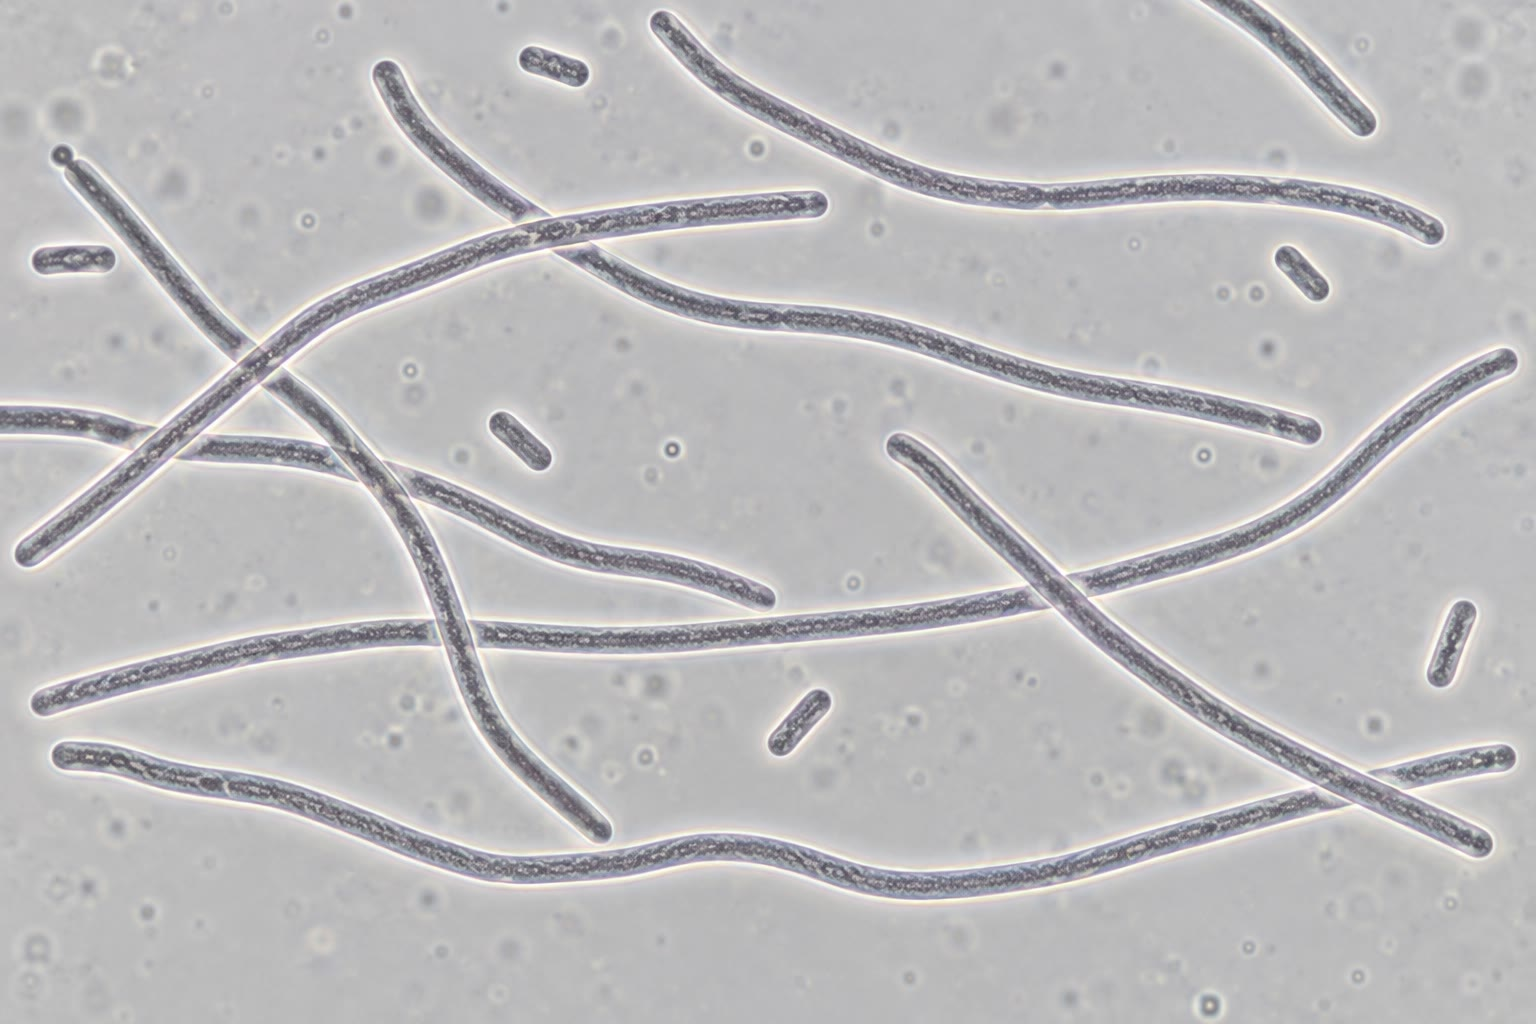
\includegraphics[width=0.46\linewidth]{images/book5/ai/b5-03-sos-filaments.jpg}\hspace{0.04\linewidth}
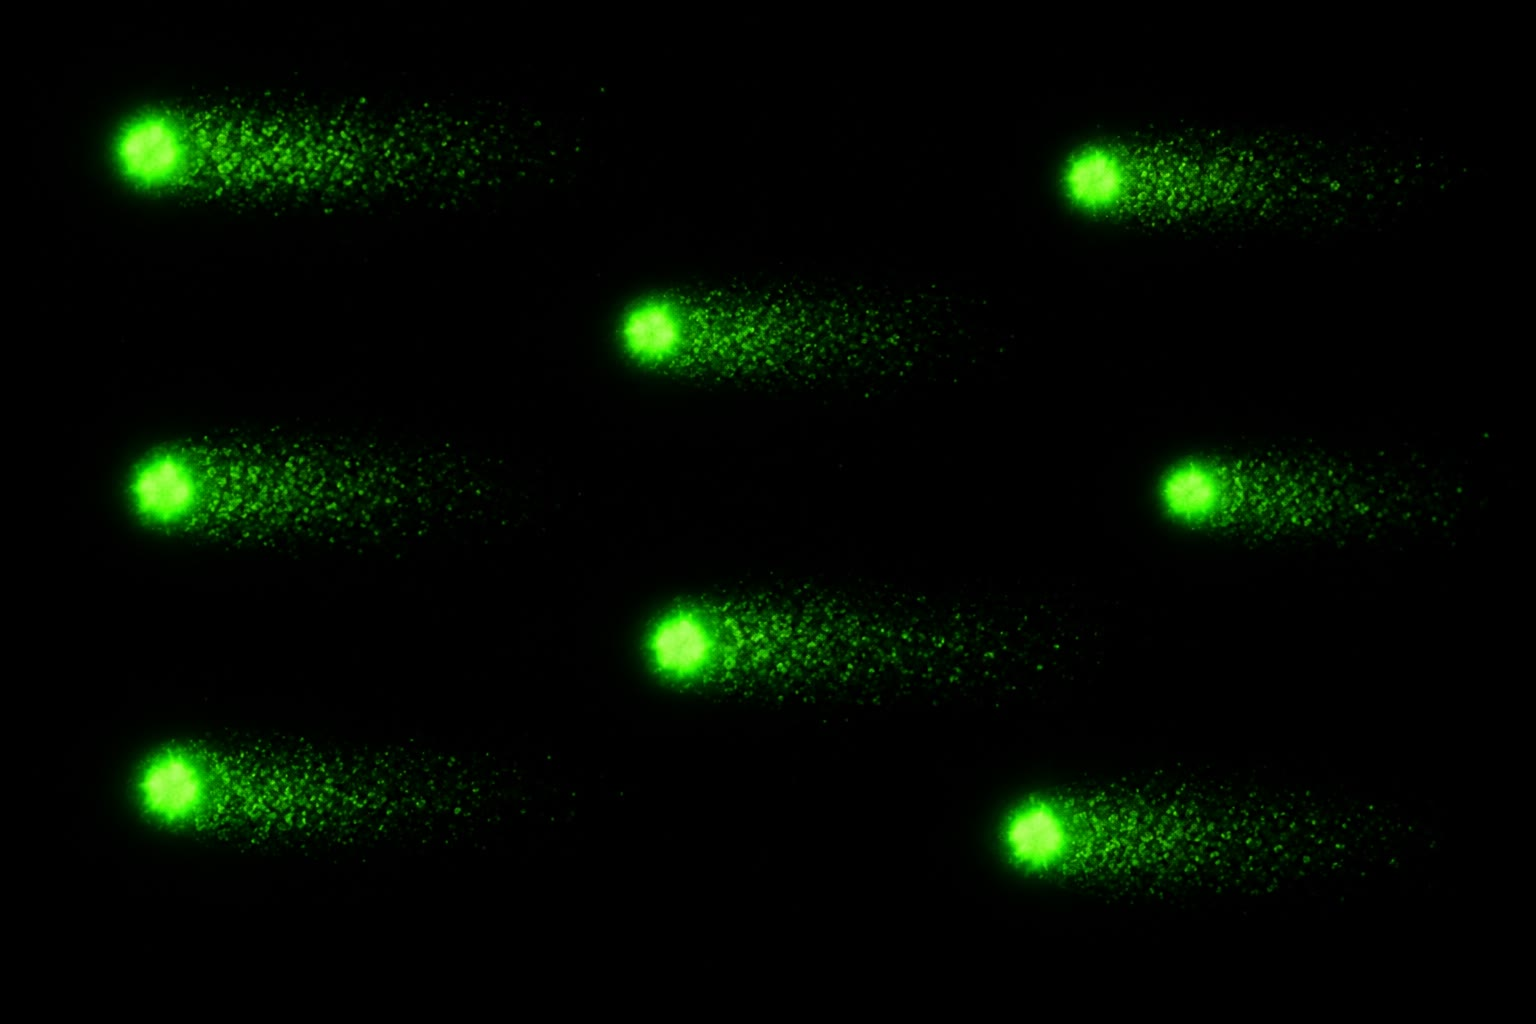
\includegraphics[width=0.46\linewidth]{images/book5/ai/b5-03-comet-assay.jpg}

{\small يسارًا: \emph{E.~coli} بعد التشعيع فوق البنفسجي، نمت
خيوطًا طويلة لأن \omterm{prop:b3:dna-repair:sos}{استجابة SOS} حجبت انقسام الخلية
ريثما يُصلح DNA. يمينًا: مقايسة المذنّب --- خلايا مفردة
تُغرس في هلام وتُرحّل كهربائيًا؛ فينساب DNA المجزأ خارج
النواة في ذيل يقيس طولُه عددَ الكسور.}
\end{omfigure}

\begin{definition}[استجابة أذية DNA]\label{def:b3:dna-repair:ddr}
\index{استجابة أذية DNA}\index{ATM}\index{نقطة تفتيش}\index{p53}\index{غاما-H2AX}
تشير حقيقيات النوى إلى الأذية بكينازين: \emph{ATM}، الذي يستدعيه
معقّد MRN إلى الكسور المزدوجة الطاق، و\emph{ATR}، الذي يُستدعى
إلى DNA المفرد الطاق عند الشوكات المتوقفة. وهما يفسفران مئات
الأهداف. وفي دقائق يُفسفر \omterm{def:b3:chromatin-epigenetics:nucleosome}{الهستون} H2AX
(\emph{$\gamma$-H2AX}) على امتداد ميغاقواعد حول كل كسر، فيتكوّن
بؤرة تستدعي بروتينات الإصلاح ويمكن عدّها تحت
المجهر، بؤرة واحدة لكل كسر. ويوقف الكينازان Chk1 وChk2
دورة الخلية --- عند \emph{نقاط التفتيش} في \cref{ch:b3:cell-cycle-apoptosis}
--- بتعطيل الفوسفاتازات التي تدفع إلى الدخول في الطور S أو
M؛ ويحرّض عامل الاستنساخ \emph{p53}، وقد ثبّتته
الفسفرة، مثبطَ الكيناز المعتمد على السيكلين p21 (فتوقف
دائم في G1)، ومورّثات الإصلاح، ومورّثات الاستماتة التي تقتل الخلية
إن كانت الأذية ثقيلة أو مستمرة. فالاستجابة تشتري
وقتًا للإصلاح، ومتى أخفق الإصلاح أزالت الخلية بدل أن
تدعها تنقسم بجينوم مكسور.
\end{definition}

\begin{omfigure}
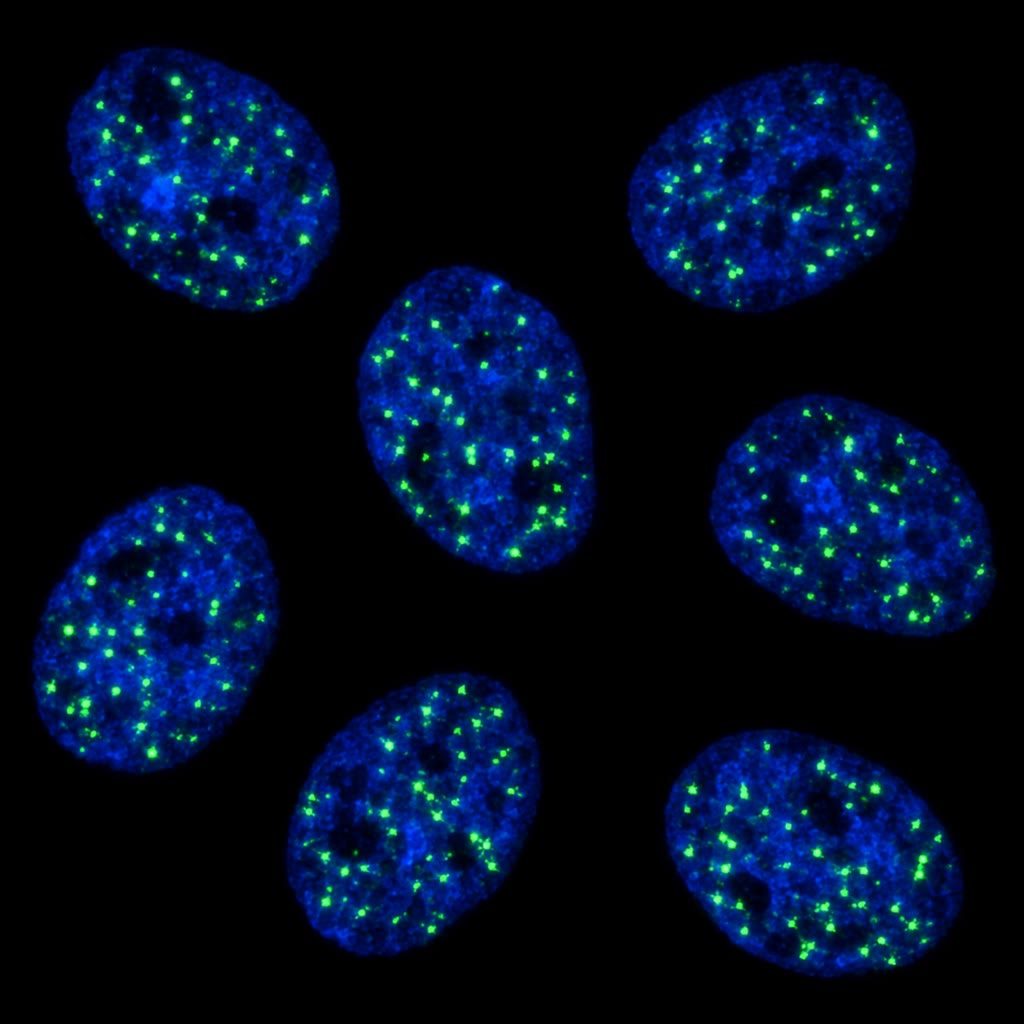
\includegraphics[width=0.4\linewidth]{images/book5/ai/b5-03-gamma-foci.jpg}

{\small بؤر $\gamma$-H2AX (بالأخضر) في أنوية (بالأزرق) بعد ساعة من
التشعيع. تعلّم كل بؤرة كسرًا مزدوج الطاق؛ وعدّها
يقيس الأذية، ويقيس إصلاحها على مدى الساعات التالية.}
\end{omfigure}

\begin{example}[الإماتة التوليفية: BRCA وPARP]\label{ex:b3:dna-repair:parp}
النساء اللواتي يرثن نسخة معطوبة من \emph{BRCA1} أو \emph{BRCA2}
خطرُ سرطان الثدي عندهن مدى العمر \qtyrange{50}{80}{\%}؛ وتنشأ
الأورام في خلايا فقدت النسخة الثانية فلم تعد
تقدر على \omterm{def:b3:dna-repair:dsb}{إعادة التركيب المتماثلة}. فتصلح تلك الخلايا
كسورها المزدوجة الطاق بوصل النهايات وحده وتتراكم فيها
إعادات الترتيب. وتكتسب أيضًا ضعفًا بعينه. فالكسور المفردة
الطاق، ونحوها \num{10000} في اليوم، تُصلَح بطريق يحتاج إلى
إنزيم PARP؛ فإذا ثبّط دواءٌ PARP، بقيت الكسور المفردة
حتى الطور S، حيث تحوّل الشوكة كلًا منها إلى \omterm{def:b3:dna-repair:lesions}{كسر مزدوج
الطاق} بنهاية واحدة --- لا يصلحه إلا إعادة التركيب. والخلية السوية،
ولها أليل \emph{\omterm{def:b3:dna-repair:dsb}{BRCA}} سليم، تتدبر أمرها؛ أما خلية الورم فتموت.
فعيبان، كلٌّ منهما بلا ضرر وحده، قاتلان معًا: فالدواء يقتل عبر
\emph{الإماتة التوليفية}، ويعفي سائر خلايا المريضة.
\end{example}

\begin{proposition}[إعادة التركيب أداةً]\label{prop:b3:dna-repair:tools}
\index{إعادة تركيب نوعية الموضع}\index{Cre-lox}
مؤشِّبات نوعية الموضع تقطع DNA وتصله عند متتاليات قصيرة محددة بلا
بحث عن تماثل ولا تركيب: فإنزيم العاثية P1
وهو Cre يعمل على مواقع \emph{loxP} بطول \qty{34}{bp}، وإنزيم
الخميرة Flp على مواقع \emph{FRT}. وموقعان في الاتجاه نفسه على جزيء
واحد يستأصلان DNA بينهما حلقةً؛ وفي اتجاهين متعاكسين
يقلبانه؛ وموقعان على جزيئين يتبادلان جناحيهما. والمورّثة
المحفوفة بموقعي \emph{loxP} (``المؤطَّرة'') لا تُحذف إلا في الخلايا
التي يُعبَّر فيها عن Cre، من مروّج يختاره المجرّب،
أو في وقت يختاره المجرّب إذا جُعل Cre فعالًا بدواء:
وهكذا تُدرس مورّثة لا غنى عنها للجنين في كبد البالغ،
أو في عصبون بعينه (\cref{ch:b3:genetic-engineering}). \omterm{def:b3:dna-repair:dsb}{وإعادة
التركيب المتماثلة} التي تملكها الخلية هي ما يستعيره الاستهداف
المورّثي والتحرير الموجَّه بمنظومة CRISPR لكتابة تسلسل مختار في
موضع مختار.
\end{proposition}

\begin{remark}[الإصلاح والشيخوخة]\label{rem:b3:dna-repair:ageing}
الخلايا التي تخفق في الإصلاح تتراكم فيها الطفرات، فتشيخ أو تموت؛
وعيوب الإصلاح الموروثة (متلازمة فيرنر، وهي هليكاز؛ ومتلازمة
كوكاين، وهي الإصلاح المقترن بالاستنساخ؛ ورنح توسع الشعيرات، وهو \omterm{def:b3:dna-repair:ddr}{ATM})
تسبب ملامح شيخوخة باكرة، ويرتفع عدد الطفرات الجسدية في الأنسجة
السوية ارتفاعًا خطيًا مع العمر بمعدل عشرات الطفرات في الخلية كل
سنة. أما هل \emph{تسبب} الأذية المتراكمة الشيخوخةَ العادية أم
تصاحبها فحسب، فأمر لم يُحسم؛ وأما أن سعة الإصلاح محدِّد لطول العمر
عبر الأنواع --- فالأنواع الأطول عمرًا تصلح أكثر --- فمدعوم دعمًا جيدًا.
\end{remark}

\section{تمارين}

\begin{exercise}[$\star$]\label{exo:b3:dna-repair:1}
صنّف هذه الآفات عفويةً أو بيئية وسمِّ مسلك إصلاح كل منها: يوراسيل في
DNA؛ وثنائي ثيمين؛ \omterm{def:b3:dna-repair:lesions}{و8-أوكسوغوانين}؛ وعدم توافق G--T خلف الشوكة؛ \omterm{def:b3:dna-repair:lesions}{وكسر
مزدوج الطاق} في الطور G1.
\end{exercise}

\begin{exercise}[$\star$]\label{exo:b3:dna-repair:2}
لماذا لا يحتاج \omterm{def:b3:dna-repair:excision}{إصلاح استئصال النوكليوتيد} إلى إنزيم خاص بكل نوع من
أنواع الآفات، بينما يحتاج \omterm{def:b3:dna-repair:excision}{إصلاح استئصال القاعدة} إلى \omterm{def:b3:dna-repair:excision}{غليكوزيلاز} لكل
نوع؟
\end{exercise}

\begin{exercise}[$\star$]\label{exo:b3:dna-repair:3}
اذكر مشكلة تمييز الطاق في \omterm{prop:b3:dna-repair:fidelity}{إصلاح عدم التوافق} وكيف تحلها
\emph{E.~coli}. وماذا يحدث في طافر \emph{dam} الذي لا يمثيل أي موقع
GATC؟
\end{exercise}

\begin{exercise}[$\star$]\label{exo:b3:dna-repair:4}
تتلقى خلية \qty{2}{Gy} من الأشعة السينية. كم كسرًا مزدوج الطاق
تصيبها تقريبًا، وكم بؤرة $\gamma$-H2AX تتوقع عدّها بعد ساعة؟ ولماذا
تقلّ بعد ست ساعات؟
\end{exercise}

\begin{exercise}[$\star\star$]\label{exo:b3:dna-repair:5}
باستعمال \cref{prop:b3:dna-repair:fidelity}، احسب معدل الطفرة لكل
زوج قواعد وعدد الطفرات الجديدة في الجينوم ثنائي الصيغة لكل انقسام في
(أ) خلية سوية، (ب) خلية تنقصها منظومة \omterm{prop:b3:dna-repair:fidelity}{إصلاح عدم التوافق}،
(ج) خلية فقد بوليميرازها نوكليازه الخارجي. وأيهما مطفِّر أخطر؟
\end{exercise}

\begin{exercise}[$\star\star$]\label{exo:b3:dna-repair:6}
تنشأ المواضع بلا قاعدة بمعدل $10^{4}$ في الخلية كل يوم وتُصلَح بعمر
نصف \qty{15}{min}. استعمل \cref{thm:b3:dna-repair:load} لتجد
عددها المستقر في الخلية. وإذا أبطأ دواءٌ الإصلاحَ عشرة أضعاف، فما
الحالة المستقرة الجديدة، وكم موضعًا تلقى الشوكة إذا نسخت الجينوم في
\qty{8}{h}؟
\end{exercise}

\begin{exercise}[$\star\star$]\label{exo:b3:dna-repair:7}
في الطور G2 يمكن إصلاح الكسر بوصل النهايات (عمر نصف \qty{30}{min}) أو
\omterm{def:b3:dna-repair:dsb}{بإعادة التركيب المتماثلة} (عمر نصف \qty{4}{h})، وكلاهما متاح. فما نسبة
الكسور التي تسلك إعادة التركيب؟ وما عمر نصف الكسور؟ ولماذا تبقى
إعادة التركيب مع ذلك هي المسلك المهم عند شوكات التضاعف المنهارة؟
\end{exercise}

\begin{exercise}[$\star\star$]\label{exo:b3:dna-repair:8}
تنبأ بسلوك السواتل المكروية، وبطيف الأورام، وبالحساسية لضوء الشمس
عند مريض به (أ) \omterm{def:b3:dna-repair:mmr}{متلازمة لينش}، (ب) \omterm{def:b3:dna-repair:excision}{جفاف الجلد المصطبغ} من الزمرة~A،
(ج) الصورة المتغايرة XP-V التي ينقصها
Pol~$\eta$.
\end{exercise}

\begin{exercise}[$\star\star$]\label{exo:b3:dna-repair:9}
موقعا \emph{loxP} في الاتجاه نفسه يحفّان بالإكسون~3 من مورّثة؛
ويُعبَّر عن Cre من مروّج لا ينشط إلا في الكبد منذ الولادة.
صِف النمط الوراثي لخلايا الكبد وللعصبونات في البالغ، وماذا يحدث
لو وُضع الموقعان في اتجاهين متعاكسين بدل ذلك.
\end{exercise}

\begin{exercise}[$\star\star\star$]\label{exo:b3:dna-repair:10}
فسّر لماذا تفتح \omterm{prop:b3:dna-repair:sos}{استجابة SOS} مورّثات الإصلاح قبل البوليميرازات
كثيرة الخطأ، مستعينًا بألفة LexA لمشغّلاتها، ولماذا قد تكون
البكتيريا التي تخلو من البوليميرازات كثيرة الخطأ أصلًا في
موقف أضعف مع ذلك في مريض يُعالج بالمضادات الحيوية.
\end{exercise}

\begin{exercise}[$\star\star\star$]\label{exo:b3:dna-repair:11}
مثبط PARP يقتل خلايا ورم معوزة \emph{\omterm{def:b3:dna-repair:dsb}{BRCA}} ولا يقتل خلايا المريضة
السوية. اعرض السلسلة السببية، ثم تنبأ بطريقتين يستطيع بهما ورم أن
يقاوم الدواء وكيف تكشف كلًا منهما.
\end{exercise}

\begin{exercise}[$\star\star\star$]\label{exo:b3:dna-repair:12}
يعطي التحويل المورّثي عند تصالب رباعيات بنسبة $3{:}1$. ارسم (أو صِف)
\omterm{def:b3:dna-repair:dsb}{وصلة هوليداي} بازدواجية متغايرة تمتد على واسم، وبيّن كيف يعطي \omterm{prop:b3:dna-repair:fidelity}{إصلاح
عدم التوافق} للازدواجية المتغايرة في أحد الاتجاهين $3{:}1$، وفي
الآخر $1{:}3$، وكيف يعطي عدمُ الإصلاح بوغًا متغاير اللواقح نفسه
(انعزال بعد الانقسام المنصّف). ولماذا يقتصر التحويل على الواسمات
القريبة من التصالب؟
\end{exercise}

\section{مسألة: يوم في حياة جينوم}

\begin{problem}[{مسألة نهاية الأسبوع --- أذية يوم واحد في خلية بشرية
معدودةً، وسلّم الأمانة مضروبًا، وجرعة شمس متابَعة إلى الشوكة في خلية
سوية وأخرى معوزة الإصلاح، وجرعة أشعة سينية مقسومة بين مسلكي إصلاح،
وضعف ورم يُحوَّل دواءً، وتنتهي إلى عدد الثنائيات التي تلقاها الشوكة،
ومعدل الطفرة لكل قاعدة، ونسبة الكسور التي تصلحها إعادة
التركيب}]
\label{pb:b3:dna-repair:1}
معطيات: للخلية البشرية ثنائية الصيغة $6.4\times 10^{9}$ زوج قواعد،
\qty{1.5}{\%} منها مشفِّرة للبروتين. والأذية العفوية في اليوم:
$10^{4}$ نزع بورين، و$400$ نزع أمين من السيتوزين، و$10^{4}$ كسر
مفرد الطاق. والأمانة: البوليميراز $10^{-5}$، والتدقيق يترك
$10^{-2}$ من الأخطاء، \omterm{prop:b3:dna-repair:fidelity}{وإصلاح عدم التوافق} $10^{-3}$. وحمام شمس يترك
$10^{5}$ ثنائي بيريميدين في الخلية الجلدية؛ وعمر نصف إصلاح
الاستئصال \qty{2}{h} في السوي و\qty{70}{h} في \omterm{def:b3:dna-repair:excision}{جفاف الجلد
المصطبغ}؛ وتصل شوكة بعد \qty{8}{h}؛ وتجاوز الثنائي بالتركيب العابر
يسبب طفرة باحتمال $10^{-3}$. وتنتج الأشعة السينية
$35$ كسرًا مزدوج الطاق لكل غراي؛ وعمر نصف وصل النهايات \qty{30}{min}،
وعمر نصف إعادة التركيب \qty{4}{h}.

\medskip
\noindent\textbf{الجزء الأول --- أيام عادية.}
\begin{enumerate}
  \item كم آفة عفوية تصيب الخلية في اليوم، وكم في السنة؟ قارن
        بحجم الجينوم.
  \item احسب معدل الطفرة لكل زوج قواعد في الانقسام، والعدد
        المتوقع من الطفرات الجديدة في الانقسام.
  \item كم من تلك الطفرات يقع في تسلسل مشفِّر للبروتين؟ وعلى مدى
        نحو $50$ انقسامًا من اللاقحة إلى خلية جلدية بالغة، كم طفرة
        مشفِّرة تحمل الخلية الجلدية من التضاعف وحده؟
  \item خلية تنقصها منظومة \omterm{prop:b3:dna-repair:fidelity}{إصلاح عدم التوافق}: ما معدل الطفرة وكم
        طفرة في الانقسام؟ والساتل المكروي ينزلق مرة في $10^{4}$
        انقسام بلا \omterm{prop:b3:dna-repair:fidelity}{إصلاح عدم التوافق} ومرة في $10^{7}$ معه.
        ففي ورم من $10^{9}$ خلية نشأ عبر $40$
        انقسامًا، كم خلية تحمل أليلًا منزلقًا عند ساتل مكروي معين
        في كل من الحالتين؟ (قدّر بالمعدل $\times$
        الانقسامات $\times$ الخلايا.)
  \item نزع أمين السيتوزين يعطي يوراسيل، ونزع أمين 5-ميثيل
        سيتوزين يعطي ثيمينًا. أيهما يُصلَح، وبماذا، وأيهما يصير
        طفرة؟ واربط ذلك بنقص \omterm{def:b3:chromatin-epigenetics:methylation}{CpG} في
        \cref{ch:b3:chromatin-epigenetics}.
  \item الغوانين المؤكسد (\omterm{def:b3:dna-repair:lesions}{8-أوكسوغوانين}) يزدوج مع A أثناء التضاعف.
        وللخلية \omterm{def:b3:dna-repair:excision}{غليكوزيلاز} يخص \omterm{def:b3:dna-repair:lesions}{8-أوكسوغوانين} قبالة C، وآخر
        يخص A قبالة \omterm{def:b3:dna-repair:lesions}{8-أوكسوغوانين}، وحلمهة تهدم dGTP المؤكسد.
        فسّر ما الذي يمنعه كل منها وأي طفرة تنتج حين تخفق
        الثلاثة.
\end{enumerate}

\medskip
\noindent\textbf{الجزء الثاني --- يوم في الشمس.}
\begin{enumerate}[resume]
  \item احسب ثابتي معدل الاستئصال $k$ في الخلية السوية وفي خلية
        جفاف الجلد.
  \item كم ثنائيًا يبقى عند الشوكة في كل منهما؟
  \item كم طفرة يسبب حمام الشمس في الخلية في كل من الحالتين، وكم
        منها في تسلسل مشفِّر؟
  \item على مدى طفولة فيها $500$ تعرض كهذا، كم طفرة مشفِّرة في
        الخلية الجلدية في كل من الحالتين؟ قارن بعدد
        التضاعف وحده في السؤال 3.
  \item نحو $20$ مورّثة، مجموع تسلسلها المشفِّر \qty{40}{kb}،
        تستطيع أن تقود سرطان جلد إذا طُفرت. فما احتمال،
        لكل خلية، أن تقع طفرة واحدة على الأقل مما يحدثه حمام
        الشمس في واحدة منها، عند طفل جفاف الجلد؟
        (استعمل بواسون بالمتوسط الصحيح.) ومع $10^{9}$ خلية معرَّضة،
        كم خلية تُصاب؟
  \item فسّر لماذا تكون مشكلة خلايا جفاف الجلد مشكلة شوكة لا مشكلة
        \omterm{def:b3:dna-repair:lesions}{الآفة} نفسها، ولماذا تظهر السرطانات في الجلد وحده.
\end{enumerate}

\medskip
\noindent\textbf{الجزء الثالث --- جرعة أشعة سينية.}
\begin{enumerate}[resume]
  \item جرعة \qty{2}{Gy}: كم كسرًا مزدوج الطاق، وكم بؤرة
        $\gamma$-H2AX بعد ساعة إذا كان وصل النهايات هو المسلك
        الوحيد (خلية في G1)؟
  \item في خلية في G2 يعمل المسلكان. احسب ثابتي المعدل
        ونسبة الكسور التي تصلحها \omterm{def:b3:dna-repair:dsb}{إعادة التركيب المتماثلة}.
  \item ما عمر نصف الكسور في G2، وكم يبقى منها
        بعد ساعة؟
  \item يغيّر كل حدث وصل نهايات بضعة أزواج قواعد عند الوصلة. فإذا
        وقعت الوصلة في تسلسل مشفِّر باحتمال $0.015$ ثم
        عطّل التغيرُ المورّثة باحتمال $0.7$،
        فكم مورّثة تعطّلها جرعة \qty{2}{Gy} في خلية G1؟
  \item مع $n$ كسرًا متزامنًا، يمكن أن توصَل النهايات خطأً فيتكون
        انتقال صبغي. فلنفترض أن كل زوج من الأزواج $n(n-1)/2$
        يوصَل خطأً باحتمال $3\times 10^{-4}$. فكم انتقالًا
        متوقعًا في الخلية عند \qty{2}{Gy}؟ وعند \qty{0.2}{Gy}؟ ولماذا
        يتناسب الخطر مع مربع الجرعة بينما يتناسب عدد
        الكسور معها خطيًا؟
  \item الجرعة \qty{2}{Gy} نفسها معطاةً على مدى \qty{10}{h} بدل
        ومضة: كم كسرًا حاضرًا في أي لحظة (الحالة
        المستقرة، وصل النهايات)؟ وماذا يعني ذلك للانتقالات
        الصبغية، ولممارسة تجزئة العلاج الشعاعي؟
  \item تنجو خلية من جرعة $D$ باحتمال $e^{-D/D_{0}}$، حيث
        $D_{0} = \qty{1.5}{Gy}$ لخلية إصلاحها سليم و
        \qty{0.5}{Gy} لخلية تنقصها منظومة وصل النهايات. احسب نجاة
        كل منهما عند \qty{2}{Gy} وعند \qty{6}{Gy}، وفسّر $D_{0}$.
\end{enumerate}

\medskip
\noindent\textbf{الجزء الرابع --- ضعف الورم.}
\begin{enumerate}[resume]
  \item خلية ورم معوزة \emph{BRCA2} تصلح كسورها بوصل النهايات وحده.
        باستعمال السؤال 14، ما نسبة كسورها في S/G2 التي تُصلَح الآن
        إصلاحًا غير دقيق وكانت الخلية السوية لتصلحها
        إصلاحًا دقيقًا؟ وماذا يفعل ذلك بجينومها على مر السنين؟
  \item يترك تثبيط PARP الكسورَ المفردة الطاق البالغة $10^{4}$
        يوميًا بلا إصلاح؛ و\qty{1}{\%} منها تحوّله الشوكات إلى كسور
        مزدوجة الطاق بنهاية واحدة. كم كسرًا كهذا في اليوم
        في الخلية، ولماذا لا يستطيع وصل النهايات إصلاح كسر بنهاية
        واحدة إصلاحًا صحيحًا؟
  \item فسّر لماذا تنجو خلايا المريضة السوية، المتغايرة اللواقح
        في \emph{BRCA2}، من الدواء.
  \item يصير ورم مقاومًا بطفرة ثانية تعيد إطار قراءة
        \emph{BRCA2}. فسّر ذلك، وقل كيف
        تكشفه.
  \item المعالجة الكيميائية بعامل مؤلكل تقتل خلايا الورم
        عبر \omterm{prop:b3:dna-repair:fidelity}{إصلاح عدم التوافق}: إذ يحاول الإنزيم إصلاح
        القواعد المؤلكلة فيطلق موت الخلية. تنبأ بأثر
        الدواء في ورم \omterm{def:b3:dna-repair:mmr}{متلازمة لينش}، الذي تنقصه منظومة \omterm{prop:b3:dna-repair:fidelity}{إصلاح عدم
        التوافق}.
  \item اذكر النتائج الثلاث: الثنائيات التي تلقاها الشوكة في خلية
        جفاف الجلد (السؤال~8)، ومعدل الطفرة السوي لكل زوج قواعد
        (السؤال~2)، ونسبة كسور G2 التي تصلحها إعادة التركيب
        (السؤال~14).
\end{enumerate}
\end{problem}
